%\RequirePackage{luatex85}
\documentclass[crop,tikz]{standalone}
\usetikzlibrary{calc,positioning,fit,arrows,arrows.meta}
\usepackage[sfdefault,light]{FiraSans}
\begin{document}

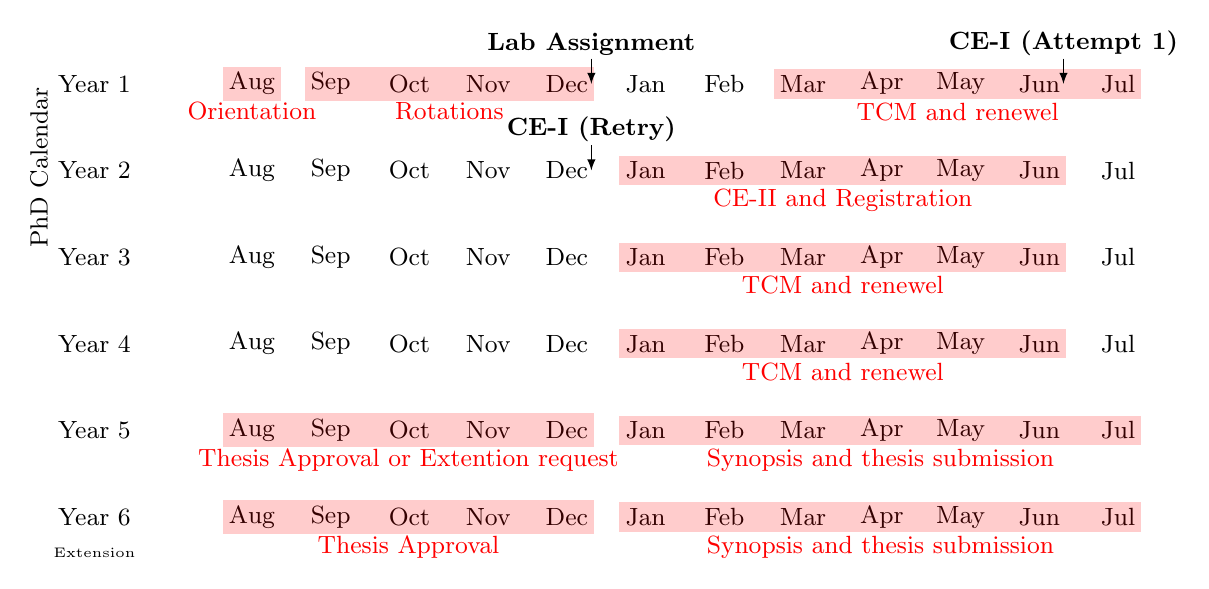
\begin{tikzpicture}[scale=1
    , every node/.style={node distance=2mm,inner sep=1pt}
]
    \small
    \edef\dy{-1.2mm}
    \edef\gap{1.1}
    \foreach \y in {1,2,3,4,5,6}
    {
        \node (year\y) at (-1,-\gap * \y cm) {Year \y};
        \foreach \month[count=\m] in {Aug,Sep,Oct,Nov,Dec,Jan,Feb,Mar,Apr,May,Jun,Jul}
        \node[] (year\y month\m) at (\m,-\gap * \y cm) {{\month}};
    }

    \node[below=of year6]{{\tiny Extension}};
    \node[left=of year1,rotate=90] {PhD Calendar};

    % Orientation.
    \def\cl{red}
    \node[fit=(year1month1),fill=\cl,opacity=0.2] (orientation) {};
    \node[below=of orientation.center] {\textcolor{\cl}{Orientation}};

    % Rotation
    \node[fill=\cl,opacity=0.2,fit= (year1month2) (year1month5) ] (rotations) { };
    \node[below=of rotations.center] {\textcolor{\cl}{Rotations}};

    \node[above=of year1month5.east,yshift=-\dy]  (labassignments) {\bf Lab Assignment};
    \draw[-latex] (labassignments) -- (year1month5.east);

    % TCM
    \node[fill=\cl,opacity=0.2,fit=(year1month8) (year1month12)] (tcm) { };
    \node[below=of tcm.center] {\textcolor{\cl}{TCM and renewel}};

    % CE
    \node[above=of year1month11.east,yshift=-\dy] (ce1) {\bf CE-I (Attempt 1)};
    \draw[-latex] (ce1) -- (year1month11.east);
    
    \node[above=of year2month5.east,yshift=-\dy] (ce2) {\bf CE-I (Retry)};
    \draw[-latex] (ce2) -- (year2month5.east);

    % Registration
    \node[fill=\cl,opacity=0.2,fit=(year2month6) (year2month11)] (reg) { };
    \node[below=of reg.center] 
        {\textcolor{\cl}{CE-II and Registration}};

    % TCM
    \node[fill=\cl,opacity=0.2,fit=(year3month6) (year3month11)] (tcm) { };
    \node[below=of tcm.center] {\textcolor{\cl}{TCM and renewel}};


    \node[fill=\cl,opacity=0.2,fit=(year4month6) (year4month11)] (tcm) { };
    \node[below=of tcm.center] {\textcolor{\cl}{TCM and renewel}};

    % Thesis 
    \node[fill=\cl,opacity=0.2,fit=(year5month1) (year5month5)] (thesis) { };
    \node[below=of thesis.center] 
        {\textcolor{\cl}{Thesis Approval or Extention request}};

    \node[fill=\cl,opacity=0.2,fit=(year5month6) (year5month12)] (thesis1) { };
    \node[below=of thesis1.center] 
        {\textcolor{\cl}{Synopsis and thesis submission}};

    % Thesis 
    \node[fill=\cl,opacity=0.2,fit=(year6month1) (year6month5)] (thesis) { };
    \node[below=of thesis.center] 
        {\textcolor{\cl}{Thesis Approval}};

    \node[fill=\cl,opacity=0.2,fit=(year6month6) (year6month12)] (thesis1) { };
    \node[below=of thesis1.center] 
        {\textcolor{\cl}{Synopsis and thesis submission}};




    


\end{tikzpicture}    

\end{document}
